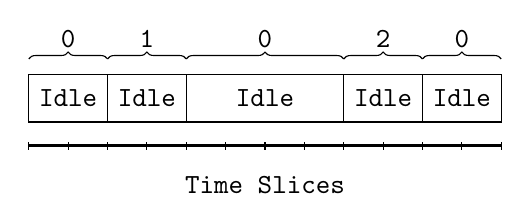
\begin{tikzpicture}[font=\ttfamily]
    % Style for general text nodes
    \tikzset{lbl/.style={inner sep=1pt, align=center}}

    % Define vertical coordinates for rows and labels
    \def\barheight{0.6} % Height of each bar
    \def\vtopprio{1.5}   % Vertical center of the top bar row
    \def\ytimeline{\vtopprio - \barheight} % Vertical position of the minor frames timeline

    % Define standard tick positions
    \def\timeslice{0.5}

    \def\astart{0}
    \def\aend{2}
    \path[draw, decorate, decoration=brace] (\astart, \vtopprio + 0.5) -- (\timeslice * \aend, \vtopprio + 0.5) node[lbl, midway, above, yshift=0.3em]{0};
    \draw (\astart, \vtopprio-\barheight/2) rectangle (\timeslice*\aend, \vtopprio+\barheight/2) 
      node[lbl, midway]{Idle};

    \def\bend{4}
    \path[draw, decorate, decoration=brace] (\timeslice * \aend, \vtopprio + 0.5) -- (\timeslice * \bend, \vtopprio + 0.5) node[lbl, midway, above, yshift=0.3em]{1};
    \draw (\timeslice * \aend, \vtopprio-\barheight/2) rectangle (\timeslice*\bend, \vtopprio+\barheight/2) 
      node[lbl, midway]{Idle};

    \def\cend{8}
    \path[draw, decorate, decoration=brace] (\timeslice * \bend, \vtopprio + 0.5) -- (\timeslice * \cend, \vtopprio + 0.5) node[lbl, midway, above, yshift=0.3em]{0};
    \draw (\timeslice * \bend, \vtopprio-\barheight/2) rectangle (\timeslice*\cend, \vtopprio+\barheight/2) 
      node[lbl, midway]{Idle};

    \def\dend{10}
    \path[draw, decorate, decoration=brace] (\timeslice * \cend, \vtopprio + 0.5) -- (\timeslice * \dend, \vtopprio + 0.5) node[lbl, midway, above, yshift=0.3em]{2};
    \draw (\timeslice * \cend, \vtopprio-\barheight/2) rectangle (\timeslice*\dend, \vtopprio+\barheight/2) 
      node[lbl, midway]{Idle};

    \def\eend{12}
    \path[draw, decorate, decoration=brace] (\timeslice * \dend, \vtopprio + 0.5) -- (\timeslice * \eend, \vtopprio + 0.5) node[lbl, midway, above, yshift=0.3em]{0};
    \draw (\timeslice * \dend, \vtopprio-\barheight/2) rectangle (\timeslice*\eend, \vtopprio+\barheight/2) 
      node[lbl, midway]{Idle};

    % Main timeline axis
    \draw[thick] (0, \ytimeline) -- (\eend*\timeslice, \ytimeline);

    % Intermediate ticks (not all but to give structure)
    \foreach \x in {0, ..., \eend} {
         \draw (\x*\timeslice, \ytimeline-0.05) -- (\x*\timeslice, \ytimeline+0.05);
    }

    % Central label below the timeline
    \node[lbl] at ( { (\eend / 2) * \timeslice }, \ytimeline-0.5 ) {Time Slices};
\end{tikzpicture}

